%\section{Result Analysis} 
\section{Laboratory Setup}
We conducted thorough testing of our developed board at Schneiders Electrical Lab. The laboratory setup is visually explained in Figure \ref{fig:x Lab}. The components labeled by red squares were employed for these tests. The TA325 flex current probe facilitated current sensing and transmission to the ADS131M08. Additionally, the Rogowski coils, coloured in red, green, and blue, were employed to sense current along the three-phase lines. Furthermore, the OMICRON CMS 356 voltage and current amplifier served as our testing equipment. It was connected to the Schneiders Real Time current and voltage simulator application. To verify current, a multimeter was utilized, and four oscilloscope probe has been connected with the acquisition board to visualise the clock, data ready, data out and sample signals.
\begin{figure}[htbp]
\centering
\includegraphics[scale=0.06]{images/LabSetup.jpg}
\caption{RMS Current measuring in Lab}
\label{fig:x Lab}
\end{figure}
\section{Calibration and Validation}
We have defined 8 calibration factors in our firmware. To put those factors we have analysed the AC current samples through our serial monitor. We have supplied 1 Amp current and found analog samples shown in figure \ref{fig:x AC Current}. 

\begin{figure}[htbp]
\centering
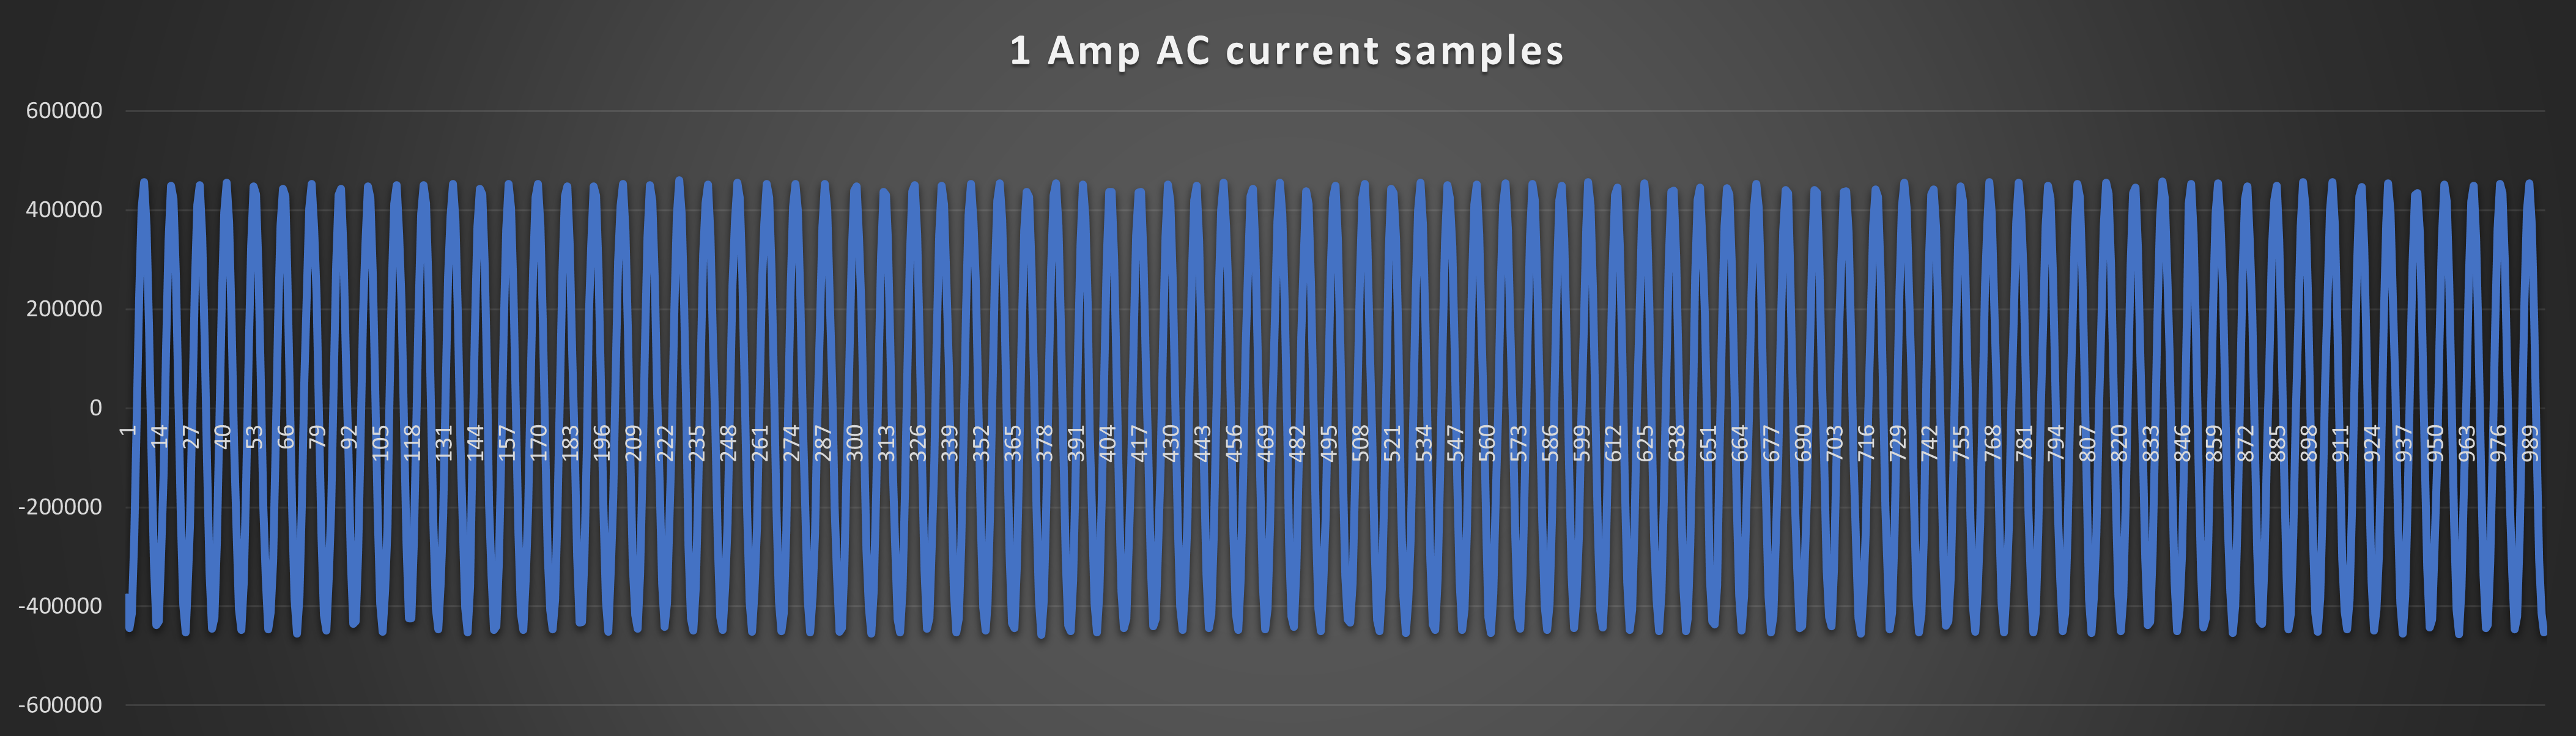
\includegraphics[scale=0.4]{images/AC_Current.png}
\caption{AC current samples}
\label{fig:x AC Current}
\end{figure}
We know that, 
\begin{align}\label{Eqn RMS}
I_{rms} = I_{peak} / \sqrt{2}
\end{align}
After analysing the AC current samples from one channel, maximum sample value was 460687. So, $I_{peak}=460687$, and applying to the equation \ref{Eqn RMS} we find the RMS value $I_{rms}=325754.9017$, what we set the calibration factor \textbf{rtU.CalI1}. Additionally, from the AC currents samples figure we can assume the data rate was approximately 4KSPS. For the voltage calibration lets have a look in figure \ref{fig:x Schematic} voltage measurement input section, each line of voltage have six 500k resistors at $V_{in}$ side, and one 4.7k resistor at $V_{out}$ side. So it makes:
\begin{align}\label{Eqn Resistance}
\frac{V_{out}}{V_{in}}=\frac{4.7k}{4.7k+3000k}=\frac{4.7k}{3004.7k}
\end{align}

Now, our reference voltage $V_{Ref}= 1.25V$, and the ADC resolution is 24 bit, as a consequence $2^{23}$ is the highest bit of ADC. We can put equation \ref{Eqn Resistance} data for making calibration voltage which will take placed by \textbf{rtU.CalV1}: 
\begin{align}\label{Eqn Cal}
V_{Cal}=\frac{V_{Ref}\times3004.7}{2^{23}\times 4.7k}
\end{align}


\section{Analysing Signal in Oscilloscope} 
\begin{figure}[htbp]
\centering
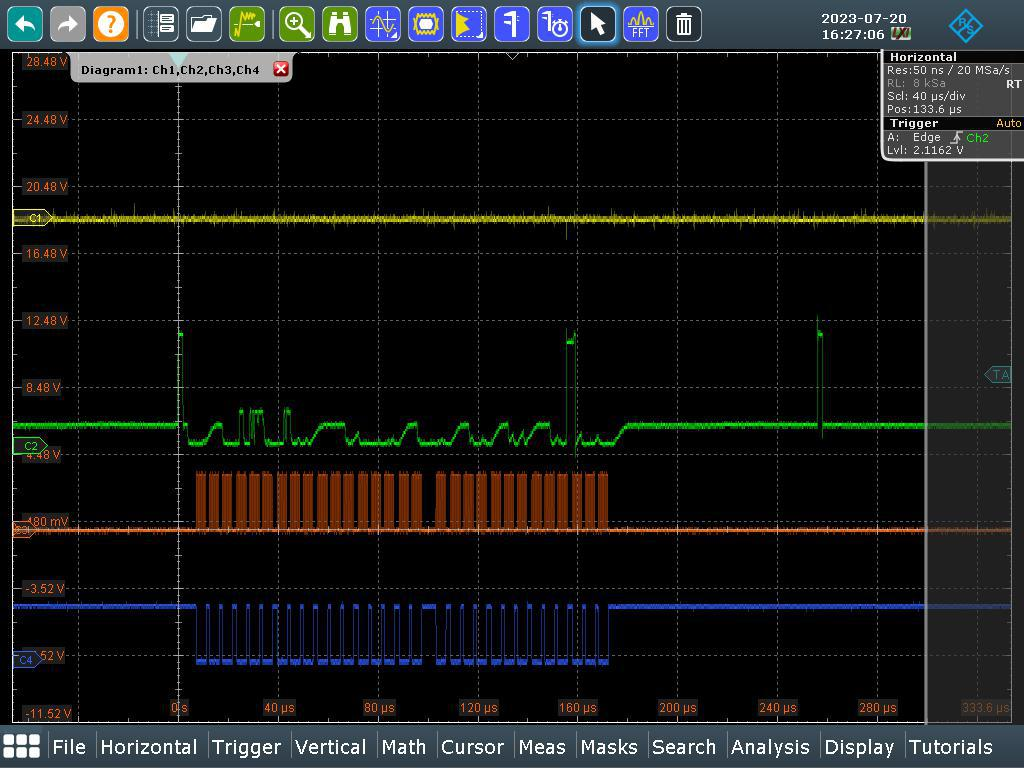
\includegraphics[scale=0.195]{images/Output 1.png}
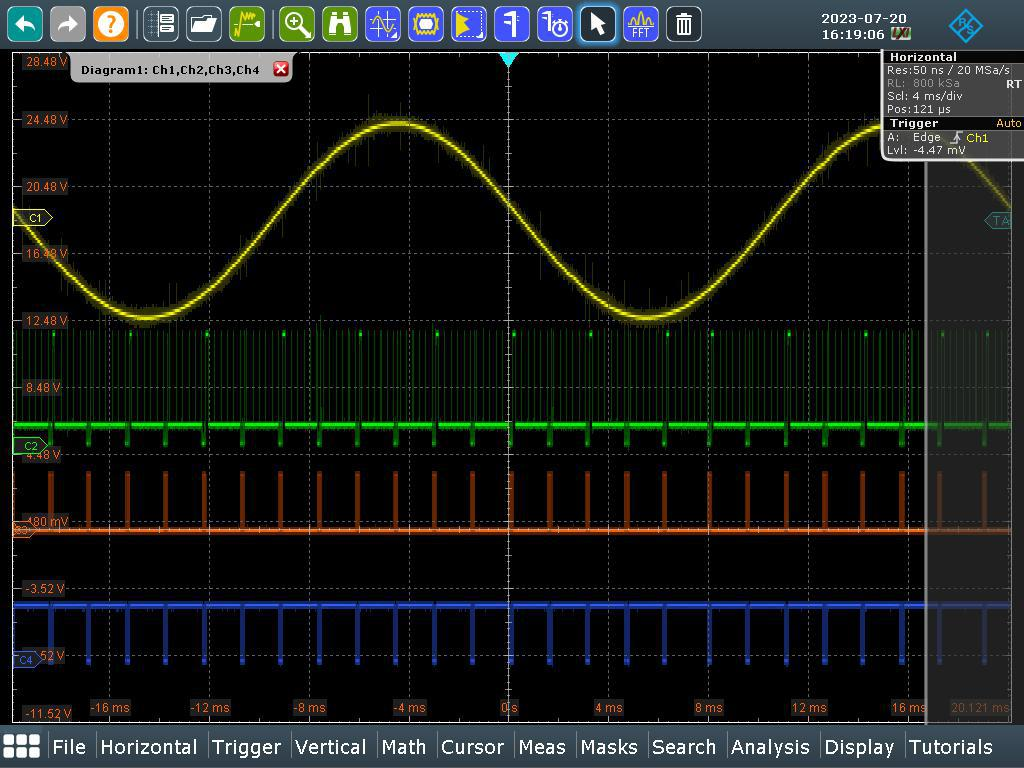
\includegraphics[scale=0.26]{images/Output 2.png}
\caption{Signals in Oscilloscope}
\label{fig:x Output1}
\end{figure}
Output from oscilloscope has been depicted in figure \ref{fig:x Output1}, where \textbf{Yellow} Signal represents Current sample (single channel), \textbf{Green} Signal represents the Data Ready, \textbf{Brown} Signal represents the master Clock, and \textbf{Blue} Signal represents the Data Output.


\section{IoT Cloud Dashboard} 
Our finalized IoT cloud dashboard is visually presented in Figure \ref{fig:x IoT_Dashboard}. The left figure showcases the RMS value within a balanced operational state, while the right figure highlights the RMS value under unbalanced conditions. Upon initiating data acquisition by pressing the dedicated button, the acquired data is synchronized at regular intervals, precisely set by us at a 1-second interval. 
\begin{figure}[htbp]
\centering
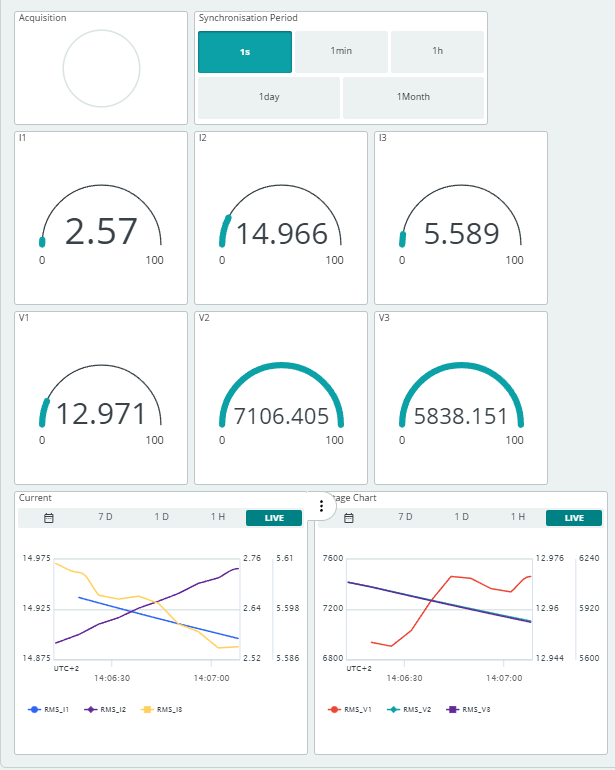
\includegraphics[scale=0.59]{images/IoT_Dashboard.png}
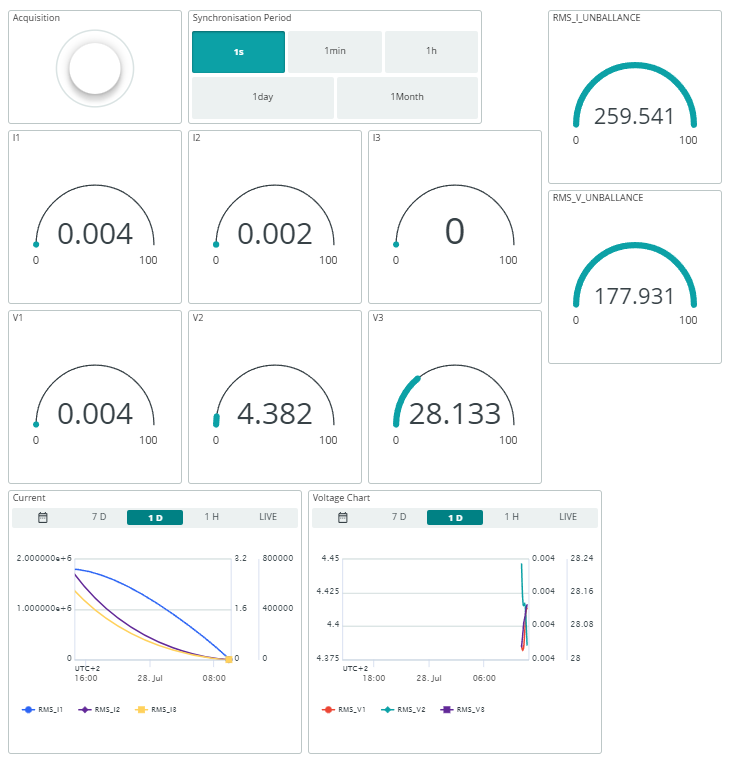
\includegraphics[scale=0.6]{images/Dashboard3.png}
\caption{Monitoring data through IoT Dashboard}
\label{fig:x IoT_Dashboard}
\end{figure}

This dynamic dashboard enables real-time monitoring of the three-phase currents (I1, I2, I3) and voltages (V1, V2, V3). Moreover, it offers intuitive graphical representations of historical data, enhancing data visualization. Notably, any instances of an unbalanced condition, expertly calculated by our system, are readily detectable through the RMS\_I\_UNBALANCE and RMS\_V\_UNBALANCE measurement units. These crucial values are meticulously computed and recorded through a dedicated local MATLAB script, overseen by our skilled engineers.

